\section*{Results and discussion}
We verified the simulation results by comparing them with physical or mathematical results known for certain potentials. The potentials analyzed are the infinite square well, barrier potential and harmonic oscillator potential.
The infinite square well finds it physical realisation in studying the behaviour of electrons confined in a metal. The barrier potential can be used as a model for understanding quantum tunneling effects. The harmonic oscillator is an ubiquitous form for the potential, finding its use mostly in approximating complex potentials near their local minima.
In two dimensions a double slit potential is used to simulate the purely quantum-mechanical effect of interference.


\subsection*{Stability of the infinite square well eigenstates}
The eigenstates of the Hamiltonian have the property that they are, up to an unphysical global phase factor, invariant under time-translations. To check the stability and accuracy of the simulation, eigenstates of the Hamiltonian for the infinite square well are simulated in two dimensions. The deviation of the wave function with its initial state is then a measure for the accuracy and stability of the simulation. It might seem intuitive to define the deviation as the distance function that is naturally induced by the inner product on the Hilbert space. However, the projective nature of the Hilbert space in quantum mechanics should be taken into account, so that a more useful approach for the deviation $D$ would be to define it as
\[
D(t) = \int\mathrm{d}x\left(|\Psi(x,t)|^2-|\Psi(x,0)|^2\right)^2,
\] where the integral is over all space.

In figures \ref{fig:distancea10}, \ref{fig:distancea05}, \ref{fig:distancea02} the eigenstate $\Psi(x,y,0) = \sin(\frac{3 \pi x}{L})\sin(\frac{2 \pi y}{L})$ is used as initial wavefunction for simulations with 500 time steps and $\tau = 1$ for $a = 1.0, 0.5$ and $0.2$ respectively. It is noted that lowering the value of $\tau$ does not affect the deviation, since the system is close to equilibrium. The value of $\tau$ only starts to play a role when there are rapid changes in the wavefunction.
\begin{Figure}
    \centering
    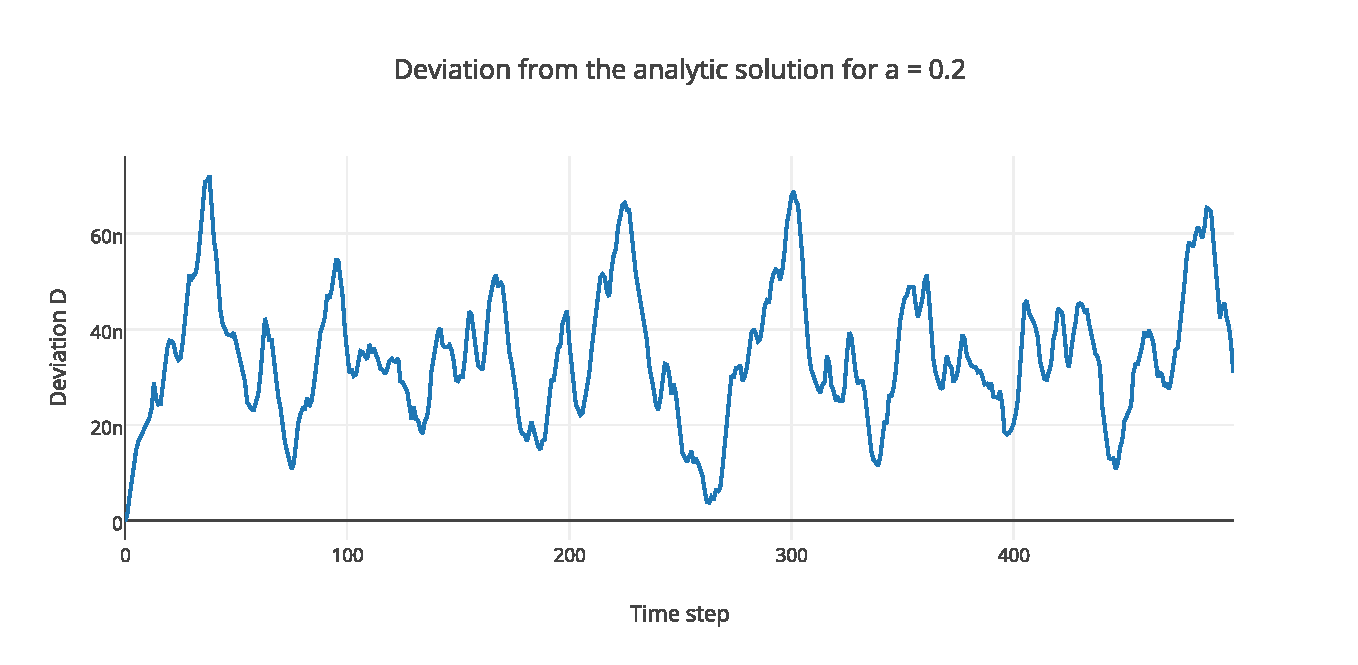
\includegraphics[width=\linewidth]{distancea10.pdf}
    \captionof{figure}{Deviation for each timestep for $a = 1.0$}
    \label{fig:distancea10}
\end{Figure}
\begin{Figure}
    \centering
    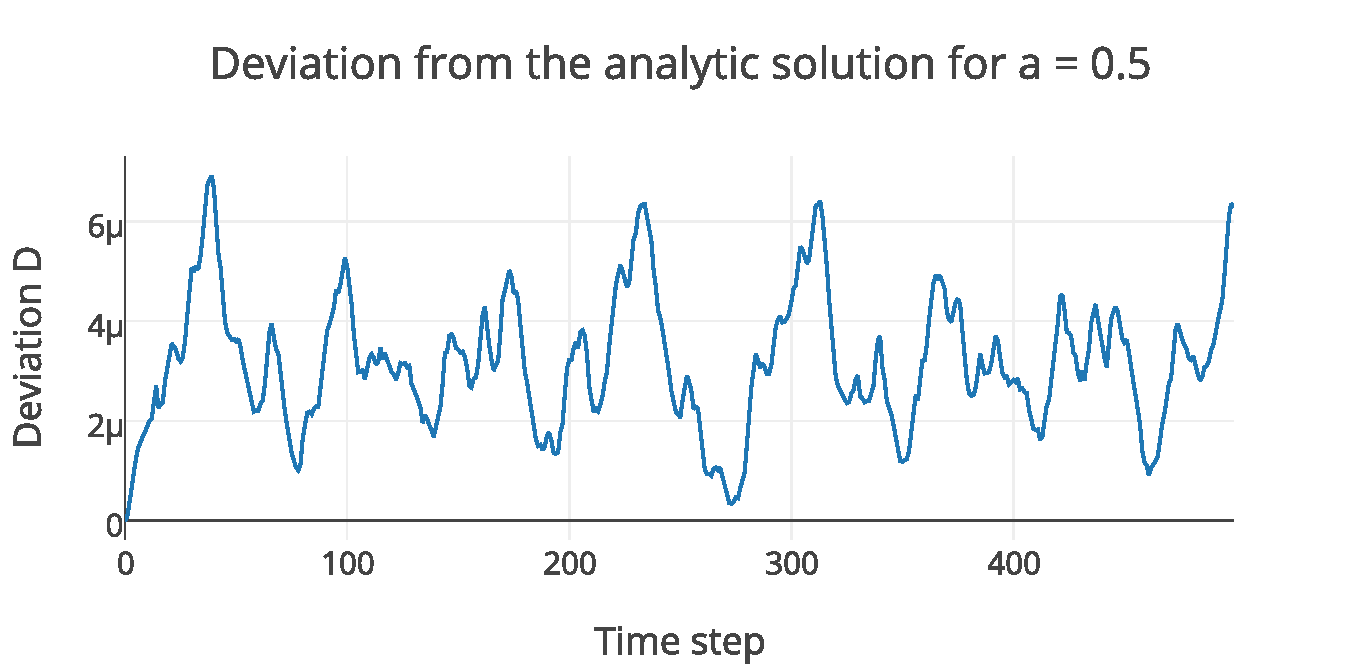
\includegraphics[width=\linewidth]{distancea05.pdf}
    \captionof{figure}{Deviation for each timestep for $a = 0.5$}
    \label{fig:distancea05}
\end{Figure}
\begin{Figure}
    \centering
    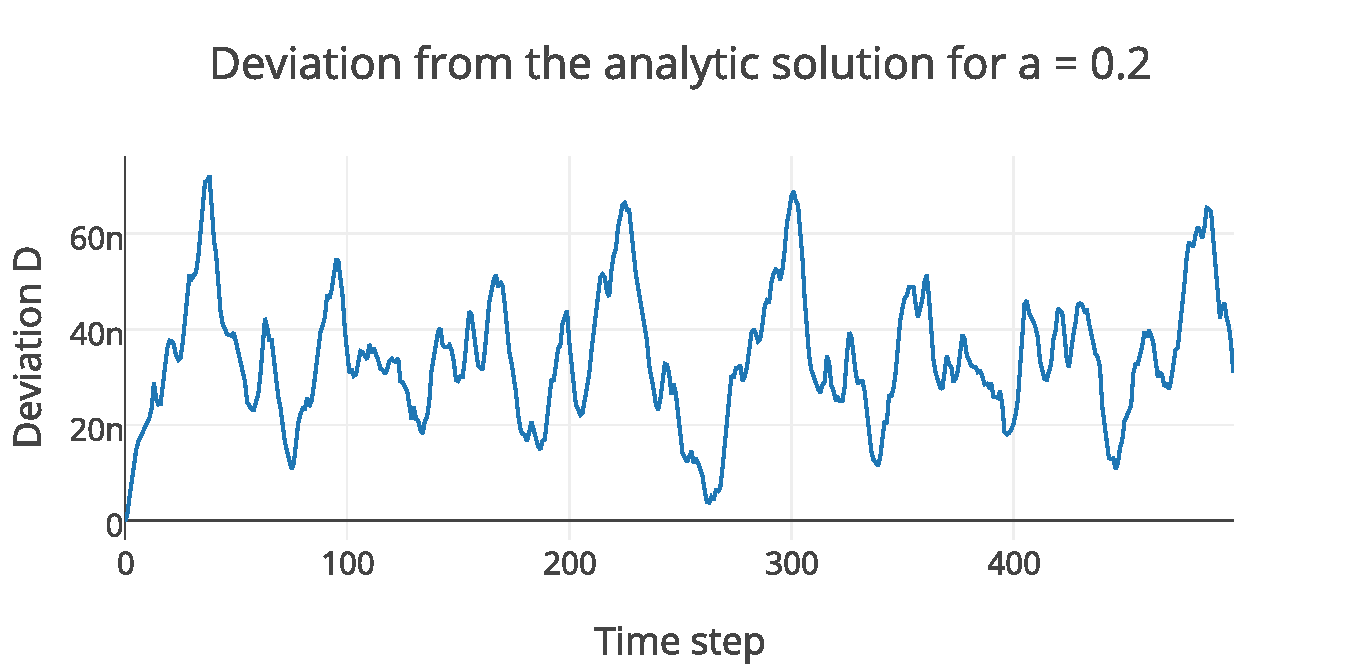
\includegraphics[width=\linewidth]{distancea02.pdf}
    \captionof{figure}{Deviation for each timestep for $a = 0.2$}
    \label{fig:distancea02}
\end{Figure} The deviations are clearly dependent on the value chosen for $a$, but the running time is expected to be around $\mathcal{O}(a^2)$, so that a proper value of $a$ should be chosen depending on the desired accuracy and running time of the simulation. The deviations occur primarily due to the fact that the analytic eigenstates of the Hamiltonian are not eigenstates of the discretized Hamiltonian\footnote{When the operator $(\mathbb{1}-\frac{i\tau}{2}\hat{H})/(\mathbb{1}+\frac{i\tau}{2}\hat{H})$ is explicitly calculated, it is possible to find approximate or exact eigenstates of the discretized Hamiltonian.}. The oscillations seen independent of $a$ indicate that the analytic eigenstate and the eigenstate of the discretized Hamiltonian are relatively close with respect to the natural metric.

\subsection*{Unitarity of the simulation}
Though the operator used in the CNM method is in theory unitary, finite precision in the storage of variables will cause the probability to be not conserved. For the following simulations the eigenstate from the previous section is simulated for 500 time steps with $\tau = 1$ and $a = 1.0, 0.5$ and $0.2$ respectively:

\begin{Figure}
    \centering
    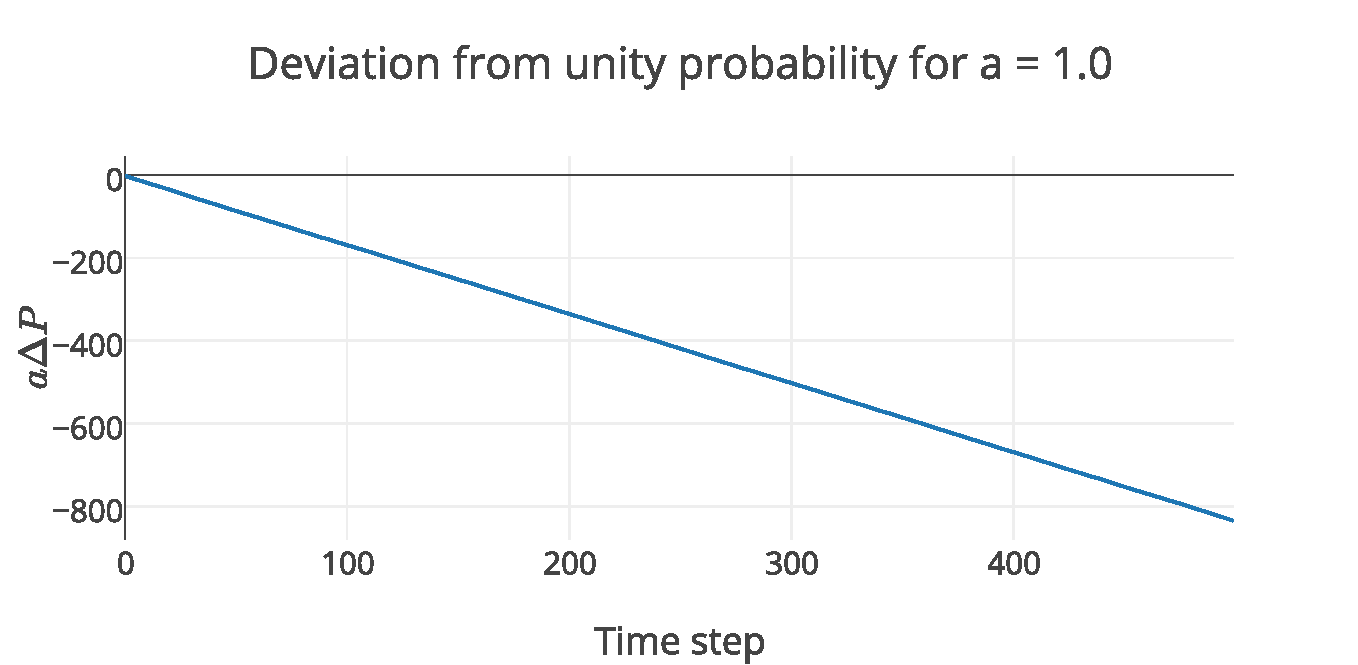
\includegraphics[width=\linewidth]{norma10.pdf}
    \captionof{figure}{Deviation from the norm for each timestep for $a = 1.0$}
    \label{fig:distancea10}
\end{Figure}

\begin{Figure}
    \centering
    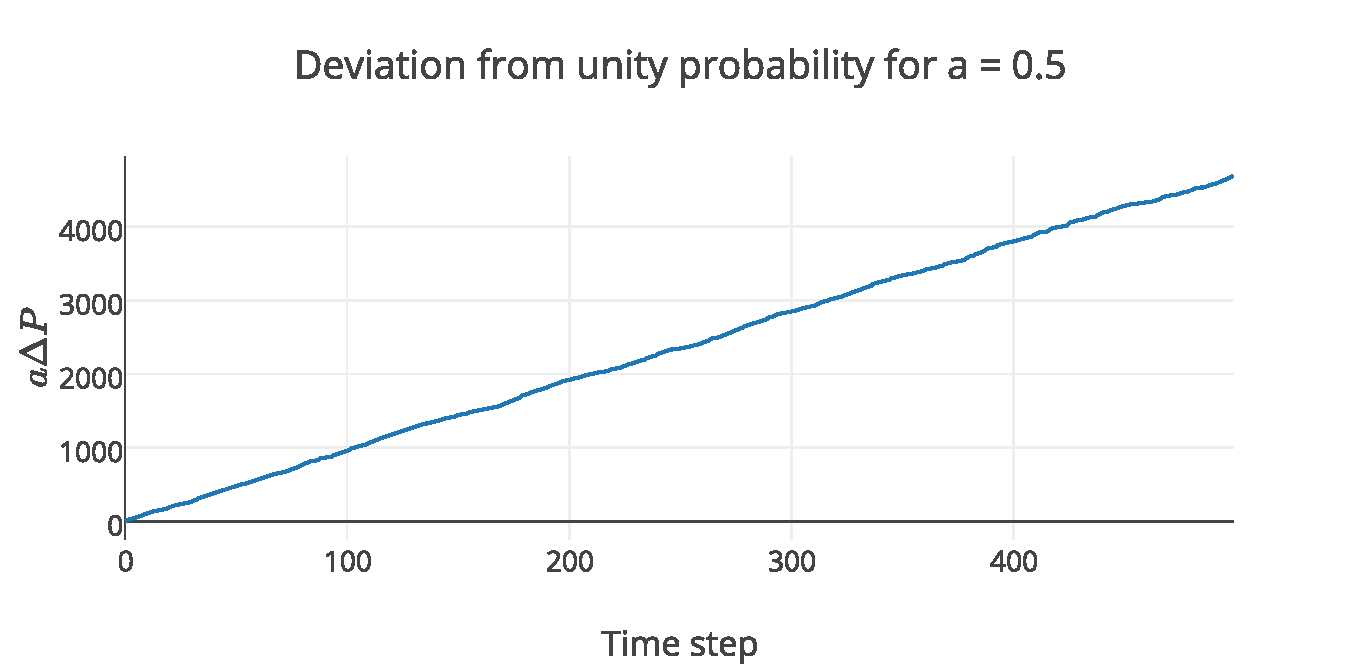
\includegraphics[width=\linewidth]{norma05.pdf}
    \captionof{figure}{Deviation from the norm for each timestep for $a = 0.5$}
    \label{fig:distancea05}
\end{Figure}

\begin{Figure}
    \centering
    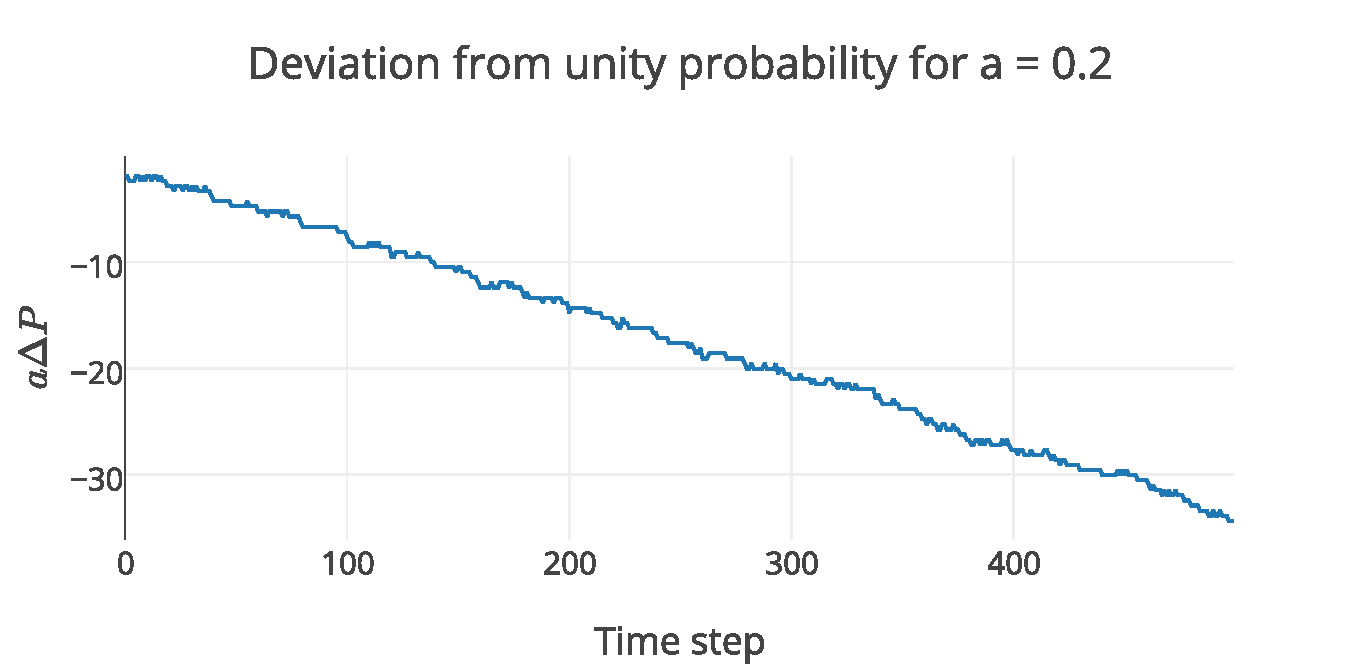
\includegraphics[width=\linewidth]{norma02.pdf}
    \captionof{figure}{Deviation from the norm for each timestep for $a = 0.2$}
    \label{fig:distancea02}
\end{Figure} The norm is seen to change linearly in time. It is clear that the total change is neglible, especially since the Schr\"{o}dinger equation and the equations solved in CNM are linear. The sudden increase in the deviation for $a=0.5$ in comparison to $a=1.0$ and $a=0.2$ could be attributed to the fact that the measure of how well a linear transformation conserves norm is not a simple function of its entries. If high precision in the absolute values of the probability is required, the wavefunctions can be renormalized after a certain amount of timesteps.

\subsection*{Transmission through a one-dimensional barrier potential}
The simulated one-dimensional barrier potential has a value $V_0>0$ in the range $40<x<42.6$ and is zero elsewhere. Sending a Gaussian wave packet through the barrier can give rise to strictly quantum mechanical effects depending on the parameters of the wave packet and the barrier. In this case, the $V_0$ is changed while the rest of the parameters are kept constant. The transmission $T$ can be calculated by integrating the probability distribution on one side of the barrier after a certain amount of tie steps.
\subsection*{Potential barrier in 1D}
\begin{Figure}
    \centering
    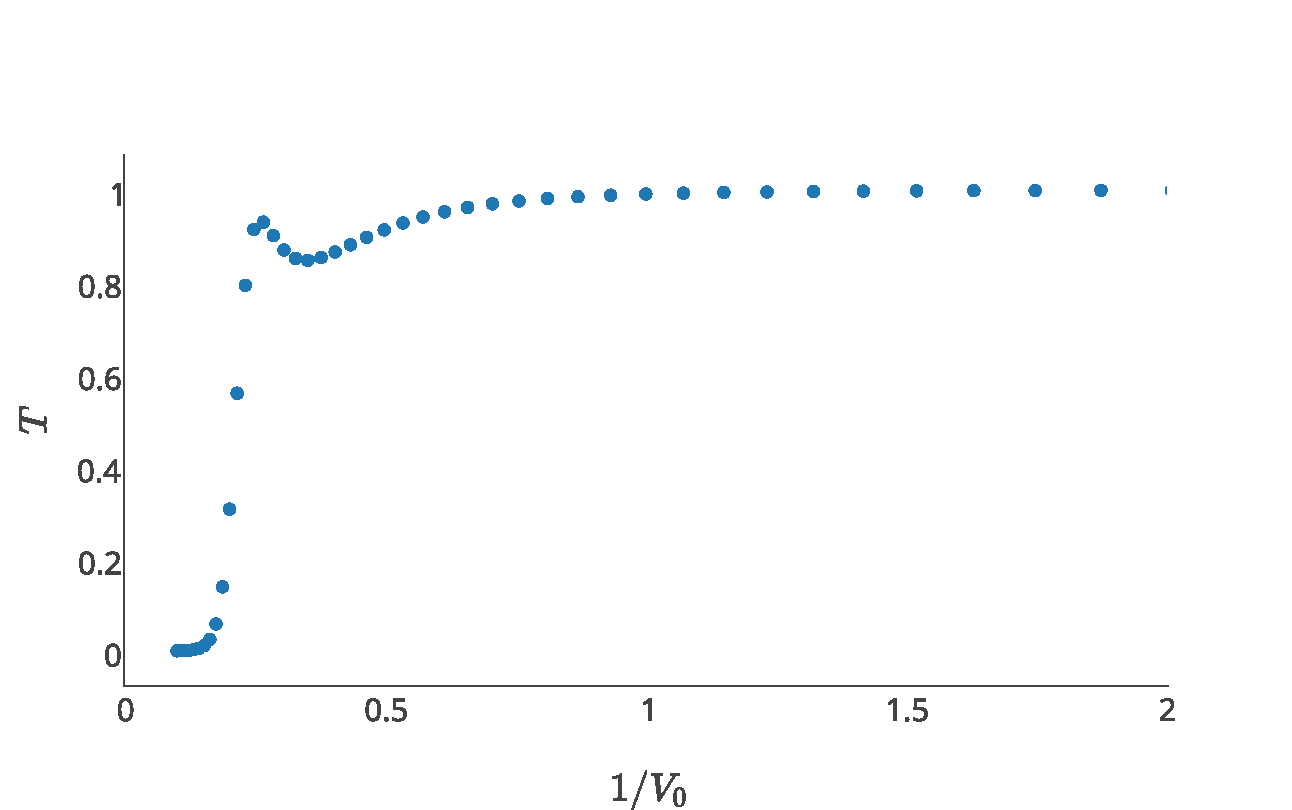
\includegraphics[width=\linewidth]{transmission_1d_pot_barrier2.pdf}
    \captionof{figure}{Transmission through a potential barrier as a function of the barrier height.}
    \label{fig:transmission}
\end{Figure} In figure \ref{fig:transmission} it can be seen that the particle tunnels partially through the barrier, even for high values of $V_0$. For low values of $V_0$ the transmission will be close to unity, as is expected. The small dip seen around $1/V_0=0.4$ is due to the wave packet resonating inside the potential barrier. This resonance effect is strongly dependent on the width of both the wave packet and the barrier.

\subsection*{Quantum harmonic oscillator potential}
The harmonic oscillator potential is defined as $V(r) = \frac{1}{2}m\omega^2r^2$, with $r$ the distance from some point in space. It is known from the classical harmonic oscillator that a particle will oscillate with a certain frequency in space. This behaviour can also be seen in the quantum analog of the harmonic oscillator. A simulation was performed by giving an offsetted Gaussian wave packet with $\sigma_x = \sigma_y = 4.5$ a momentum in the positive x-direction in a harmonic potential with $\omega = 0.2$ on a domain of 40 by 40. Snapshots evenly spread out over the duration of 150 time steps with $\tau = 0.5$ and $a = 0.5$ are shown in figure \ref{fig:QHO}
\def\arraystretch{0.6}%
\setlength\tabcolsep{0.5mm}
\begin{figure}[H]
\centerfloat
\begin{tabular}{ccc}
  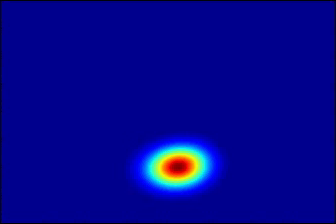
\includegraphics[scale = 0.29]{QHO1.png}  &   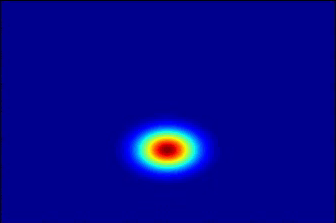
\includegraphics[scale = 0.29]{slit2.png}   &   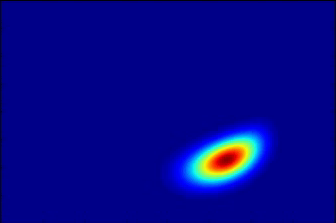
\includegraphics[scale = 0.29]{QHO3.png} \\
  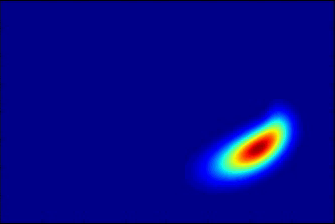
\includegraphics[scale = 0.29]{QHO4.png}  &   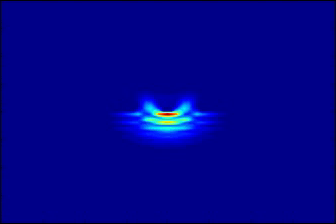
\includegraphics[scale = 0.29]{slit5.png}   &   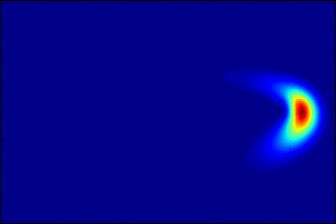
\includegraphics[scale = 0.29]{QHO6.png} \\
  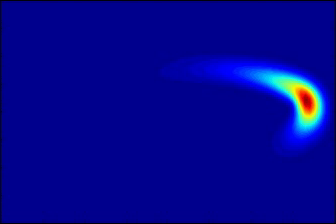
\includegraphics[scale = 0.29]{QHO7.png}  &   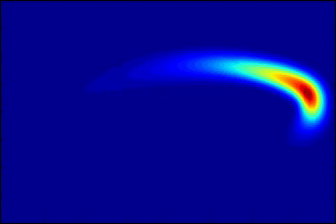
\includegraphics[scale = 0.29]{QHO8.png}    &   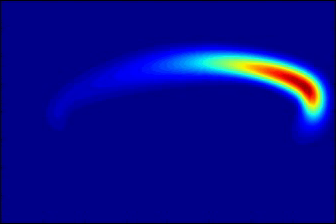
\includegraphics[scale = 0.29]{QHO9.png} \\
  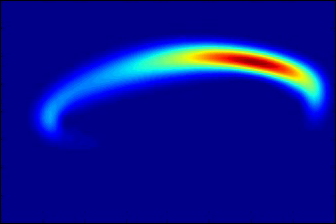
\includegraphics[scale = 0.29]{QHO10.png} &   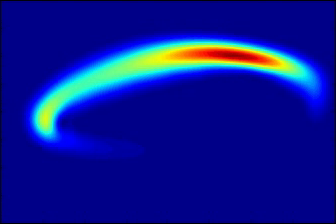
\includegraphics[scale = 0.29]{QHO11.png}   &   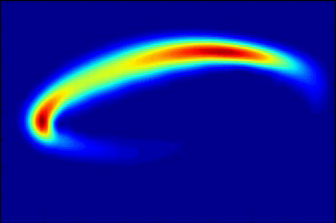
\includegraphics[scale = 0.29]{QHO12.png} \\
  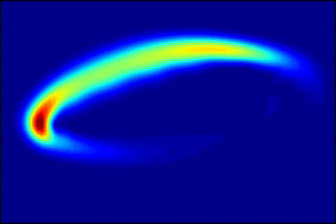
\includegraphics[scale = 0.29]{QHO13.png} &   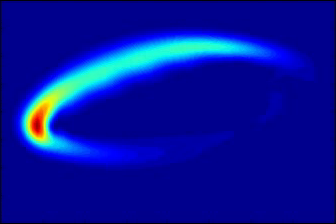
\includegraphics[scale = 0.29]{QHO14.png}   &   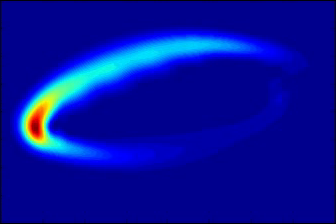
\includegraphics[scale = 0.29]{QHO15.png} \\
\end{tabular}
\caption{Time-evolution of a moving Gaussian wave packet in a harmonic potential. From left to right.}
\label{fig:QHO}
\end{figure} Note that the spread in the wavefunction increases the closer the expectation value gets to the centre of the potential. This corresponds to the behaviour of the classical harmonic oscillator where the momentum is greatest as the particle moves through the centre, while the momentum is zero as it reaches its farthest point from the centre.

\subsection*{Double slit potential}
A Gaussian wave packet with $\sigma_x = \sigma_y = 4.5$ is sent through a potential barrier with height $V_0 = 100$, with two regions of width 3 in the barrier where the potential is set to zero. The wavefunction will partially spread from these two slits and create an interference pattern on the other side. Twelve snapshots spread out evenly over 80 time steps with $\tau = 0.1$ and $a=0.5$ are shown in figure \ref{fig:doubleslit}. The simulation takes place on a domain of 40 by 40.\footnote{Animations of these simulations can be viewed on: \text{ }\url{https://github.com/dbouman1/iccp-assignment-3/tree/2D/videos}}:


%
%\begin{figure}
%  \centering
%  \raisebox{35pt}{\parbox[b]{.1\textwidth}{labelA}}%
%  \subfloat[][]{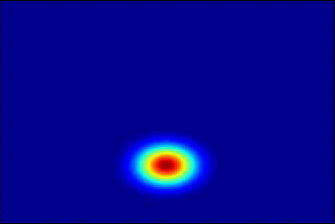
\includegraphics[width=.28\textwidth]{slit1}}\hfill
%  \subfloat[][]{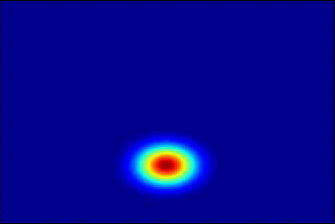
\includegraphics[width=.28\textwidth]{slit1.png}}\hfill
%  \subfloat[][]{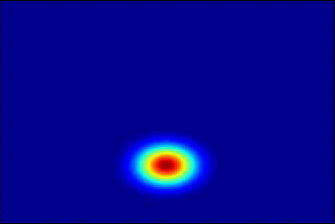
\includegraphics[width=.28\textwidth]{slit1.png}}\par
%  \raisebox{35pt}{\parbox[b]{.1\textwidth}{labelB}}%
%  \subfloat[][]{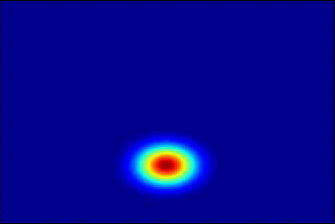
\includegraphics[width=.28\textwidth]{slit1.png}}\hfill
%  \subfloat[][]{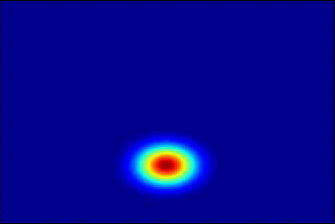
\includegraphics[width=.28\textwidth]{slit1.png}}\hfill
%  \subfloat[][]{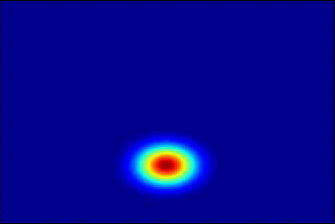
\includegraphics[width=.28\textwidth]{slit1.png}}\par
%  \raisebox{35pt}{\parbox[b]{.1\textwidth}{labelC}}%
%  \subfloat[][]{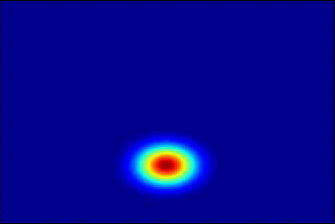
\includegraphics[width=.28\textwidth]{slit1.png}}\hfill
%  \subfloat[][]{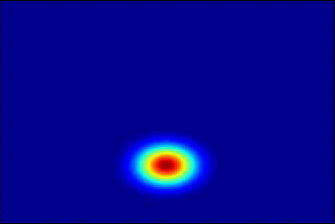
\includegraphics[width=.28\textwidth]{slit1.png}}\hfill
%  \subfloat[][]{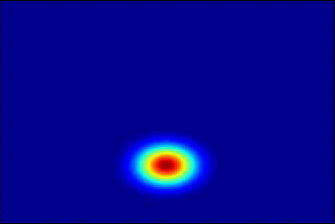
\includegraphics[width=.28\textwidth]{slit1.png}}
%  \caption{Fields}
%  \label{subplots1310}
%\end{figure}
\def\arraystretch{0.6}%
\setlength\tabcolsep{0.5mm}
\begin{figure}[H]
\centerfloat
\begin{tabular}{ccc}
  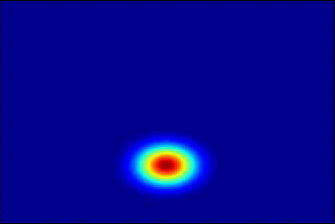
\includegraphics[scale = 0.29]{slit1.png} &   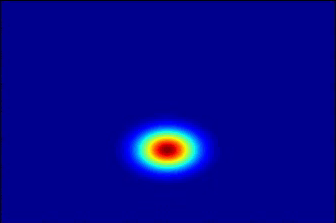
\includegraphics[scale = 0.29]{slit2.png} &   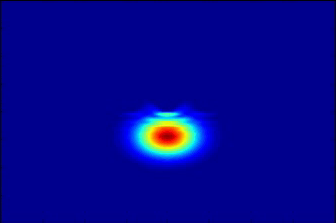
\includegraphics[scale = 0.29]{slit3.png} \\
  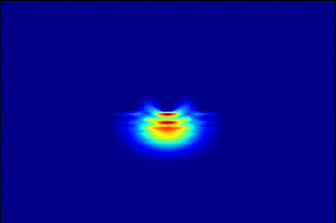
\includegraphics[scale = 0.29]{slit4.png} &   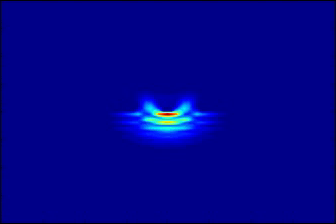
\includegraphics[scale = 0.29]{slit5.png} &   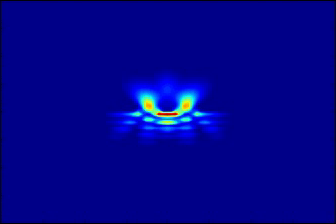
\includegraphics[scale = 0.29]{slit6.png} \\
  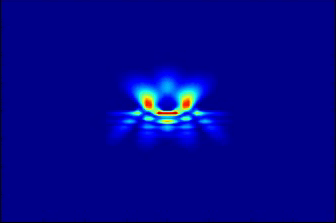
\includegraphics[scale = 0.29]{slit7.png} &   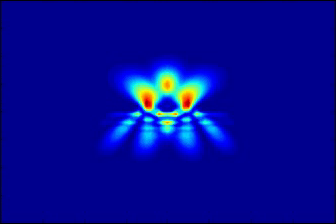
\includegraphics[scale = 0.29]{slit8.png} &   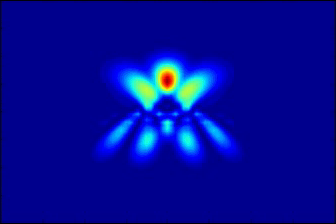
\includegraphics[scale = 0.29]{slit9.png} \\
  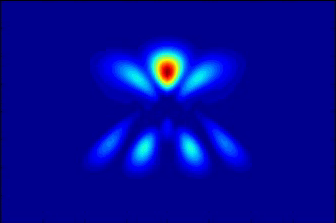
\includegraphics[scale = 0.29]{slit10.png} &   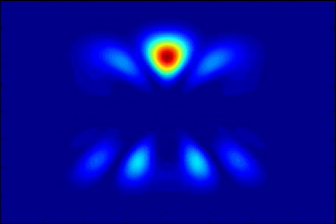
\includegraphics[scale = 0.29]{slit11.png} &   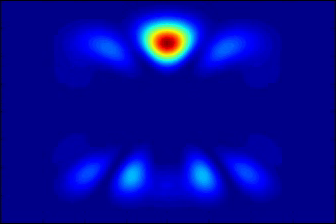
\includegraphics[scale = 0.29]{slit12.png} \\
\end{tabular}
\caption{Time-evolution of a Gaussian wave packet through a double slit. From left to right.}
\label{fig:doubleslit}
\end{figure} Figure \ref{fig:crosssection} shows a cross-section along the x-axis at $y = 26.5$, $t = 60$, $\tau = 0.1$ of the probability distribution is seen figure \ref{fig:doubleslit}. The probability distribution is again normalized to find the conditional distribution:

\begin{Figure}
    \centerfloat
    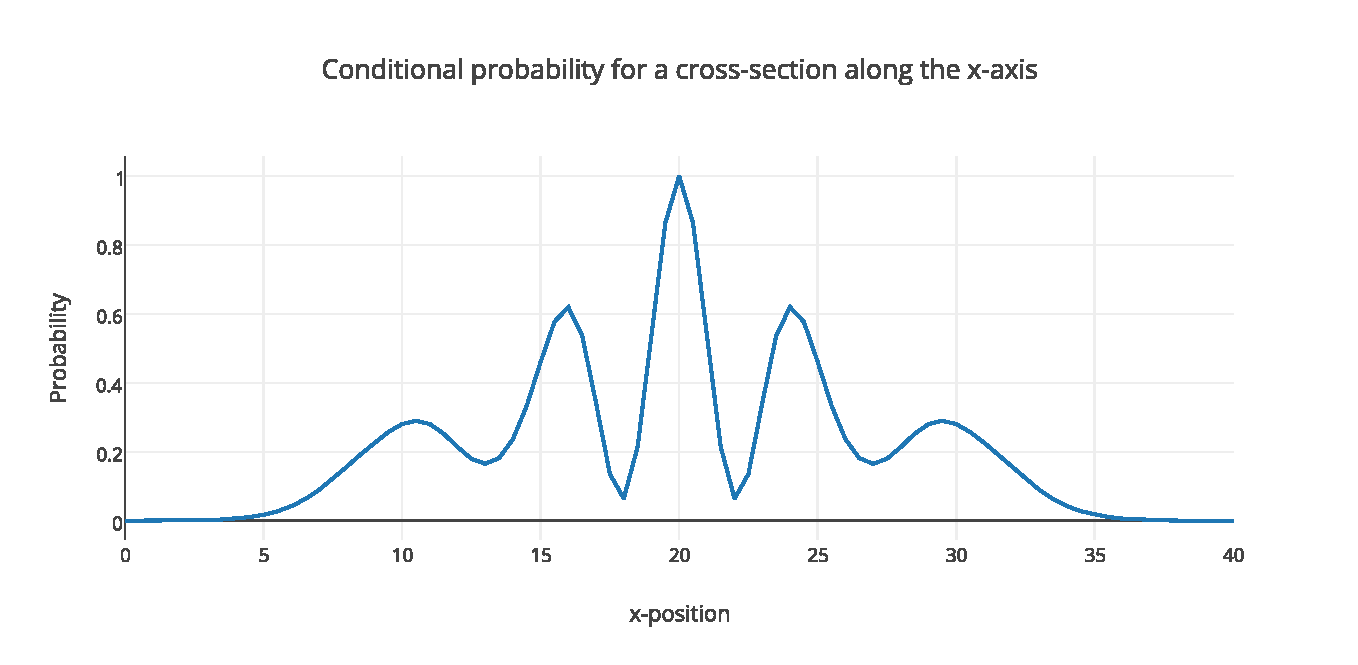
\includegraphics[trim = 3.5mm 0mm 3.5mm 0mm, clip,scale = 0.395]{crosssectiondoubleslit.pdf}
    \captionof{figure}{Conditional probability distribution for $y = 26.5$ at $t = 60$.}
    \label{fig:crosssection}
\end{Figure}
